\documentclass{beamer}

%\usetheme{Boadilla}%personally, none of the presets suit well in this case
\usecolortheme{lily}

%\usepackage[hangul]{kotex}%to input Korean letters
%including the above package widens the gap between lines
%\usepackage{fancyvrb}%fancy verbatim
\usepackage{color}%to use color presets
\usepackage{graphicx}%includegraphics

\setbeamertemplate{navigation symbols}{}%to suppress navigation tools
\setbeamertemplate{footline}[text line]{%
	\parbox{\linewidth}{\vspace*{-8pt}201601 ScienceInNarratives\hfill\hfill\insertpagenumber}}%footer

\renewcommand{\baselinestretch}{1.3}

\begin{document}
	
	% title slide
	\begin{frame}
		\title{Narrative Story Analysis : Not Enough Room!}
		\author{14080 Sangheon Lee}
		\date{2016.03.30}
		\titlepage
	\end{frame}
	
	%outline slide
	\section*{Table of contents}
	\begin{frame}
		\frametitle{Table of contents}
		\setcounter{tocdepth}{1}
		\tableofcontents
	\end{frame}
	
	\section*{Preliminaries}
	\begin{frame}
		\frametitle{Preliminaries}
		\begin{itemize}
			\item This file analyzes a story, `Not Enough Room'.
			\item This file contains massive text. I sincerely apologize for the lack of abstraction.
			\item If understood, go on to the next page where the analysis starts.
		\end{itemize}
	\end{frame}
	
	\begin{frame}
		\frametitle{Not Enough Room!}
		\begin{figure}
			\centering
			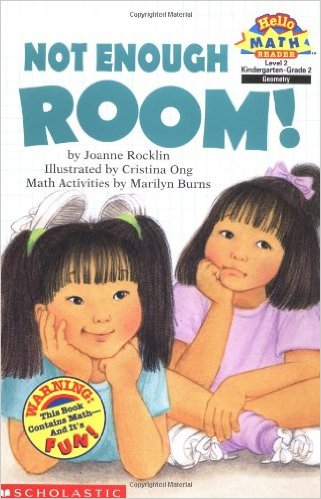
\includegraphics[scale=0.3]{res/cover.jpg}
			%http://ecx.images-amazon.com/images/I/51XBIdoDHoL._SX319_BO1,204,203,200_.jpg
		\end{figure}
		\centering
		The cover of the book.
	\end{frame}
	
	\setcounter{section}{0}
	
	\section{Section 1 : Character}\label{sec:character}%The name of sections are ASCII
	\begin{frame}
		\frametitle{Section \ref{sec:character} : Character}
		There are four characters in this story.
		\begin{itemize}
			\item Pat : The storyteller who had her own room.
			\item Kris : The storyteller's sister who also had her own room.
			\item Mom : The siblings' mother.
			\item Baby : The sibling's baby, though no direct appearance is made.
		\end{itemize}
	\end{frame}
	
	\begin{frame}
		\frametitle{Section \ref{sec:character} : Character}
		\begin{figure}
			\centering
			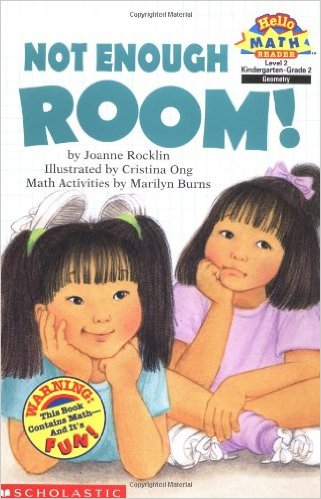
\includegraphics[scale=0.3]{res/cover.jpg}
		\end{figure}
		The girl wearing a blue T-shirt is Pat, while the girl with the purple ribbon on her head is Pat's sister, Kris.
	\end{frame}
	
	\begin{frame}
		\frametitle{Section \ref{sec:character} : Character}
		As we will discover, there is no {\color{cyan} antagonist} in this story, while the confilct does exist.
	\end{frame}
	
	\section{Section 2 : Settings}\label{sec:settings}
	\begin{frame}
		\frametitle{Section \ref{sec:settings} : Settings}
		The basic settings of this story are:
		\begin{itemize}
			\item Place : The siblings' house. Especially, their {\bf room}.
			\item Time : Once upon a time - there is no specific description.
			\item Social conditions : The siblings are kind to each other.
			%\item Mood : A mildly challenging spirit innately exists.
		\end{itemize}
	\end{frame}
	
	\section{Section 3 : Plot}\label{sec:plot}
	\begin{frame}
		\frametitle{Section \ref{sec:plot} : Plot}
		We will analyze the plot by five components:
		\begin{itemize}
			\item Main character's wish
			\item Obstacle's problem
			\item Sequence of events
			\item Climax
			\item Resolution
		\end{itemize}
	\end{frame}
	
	\begin{frame}
		\frametitle{Section \ref{sec:plot} : Plot}
		\framesubtitle{1. Main character's wish}
		\begin{itemize}
			\item The main wish of Pat and Kris is {\color{cyan} to have their own space in a comfortable manner}.
			\item It was fine since they had their own room {\bf until}......
		\end{itemize}
		\begin{figure}
			\centering
			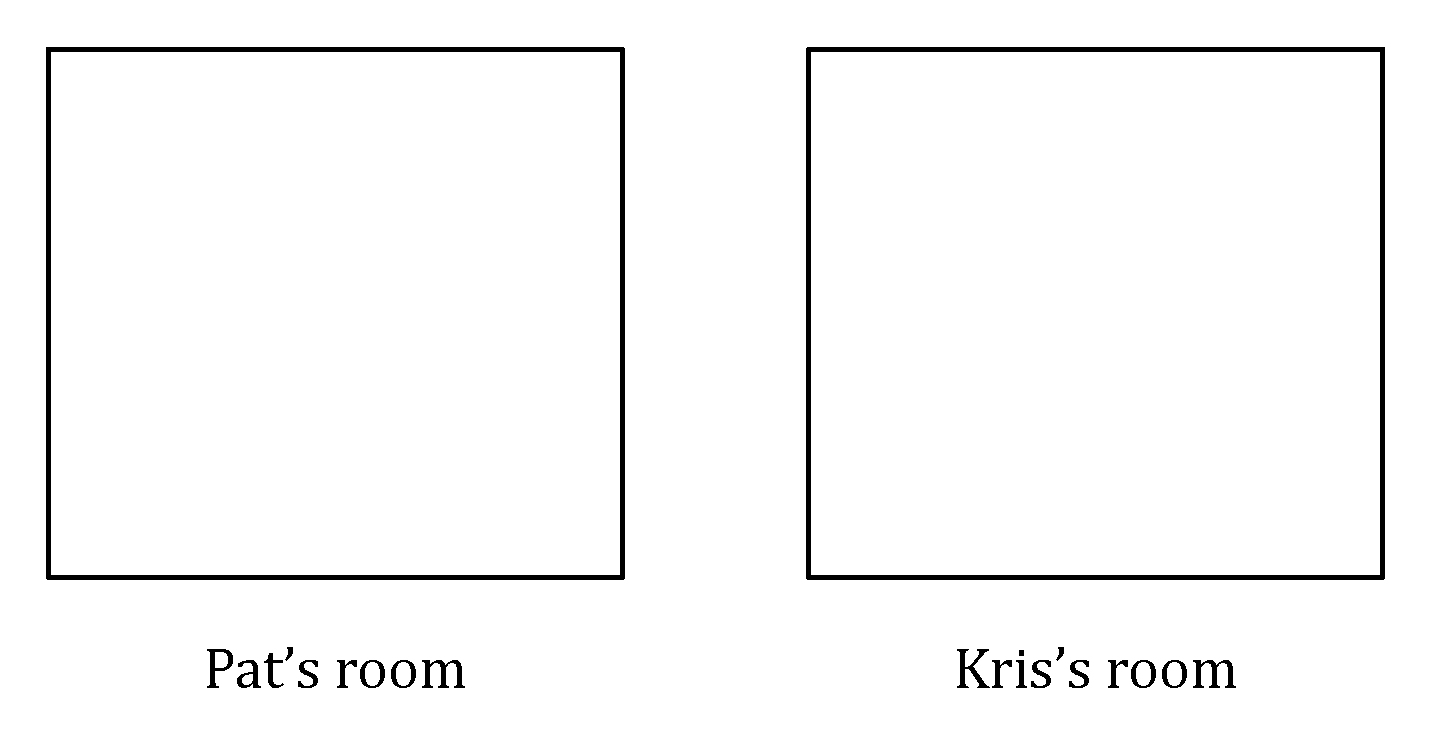
\includegraphics[width=0.6\textwidth]{res/room1_cropped.pdf}
		\end{figure}
	\end{frame}
	
	\begin{frame}
		\frametitle{Section \ref{sec:plot} : Plot}
		\framesubtitle{2. Obstacle's problem}
		\begin{itemize}
			\item ......until baby came to their house.
			\item So they had to share their rooms.
			\item But as we can easily guess, they wanted {\bf their} own space. 
		\end{itemize}
		\begin{figure}
			\centering
			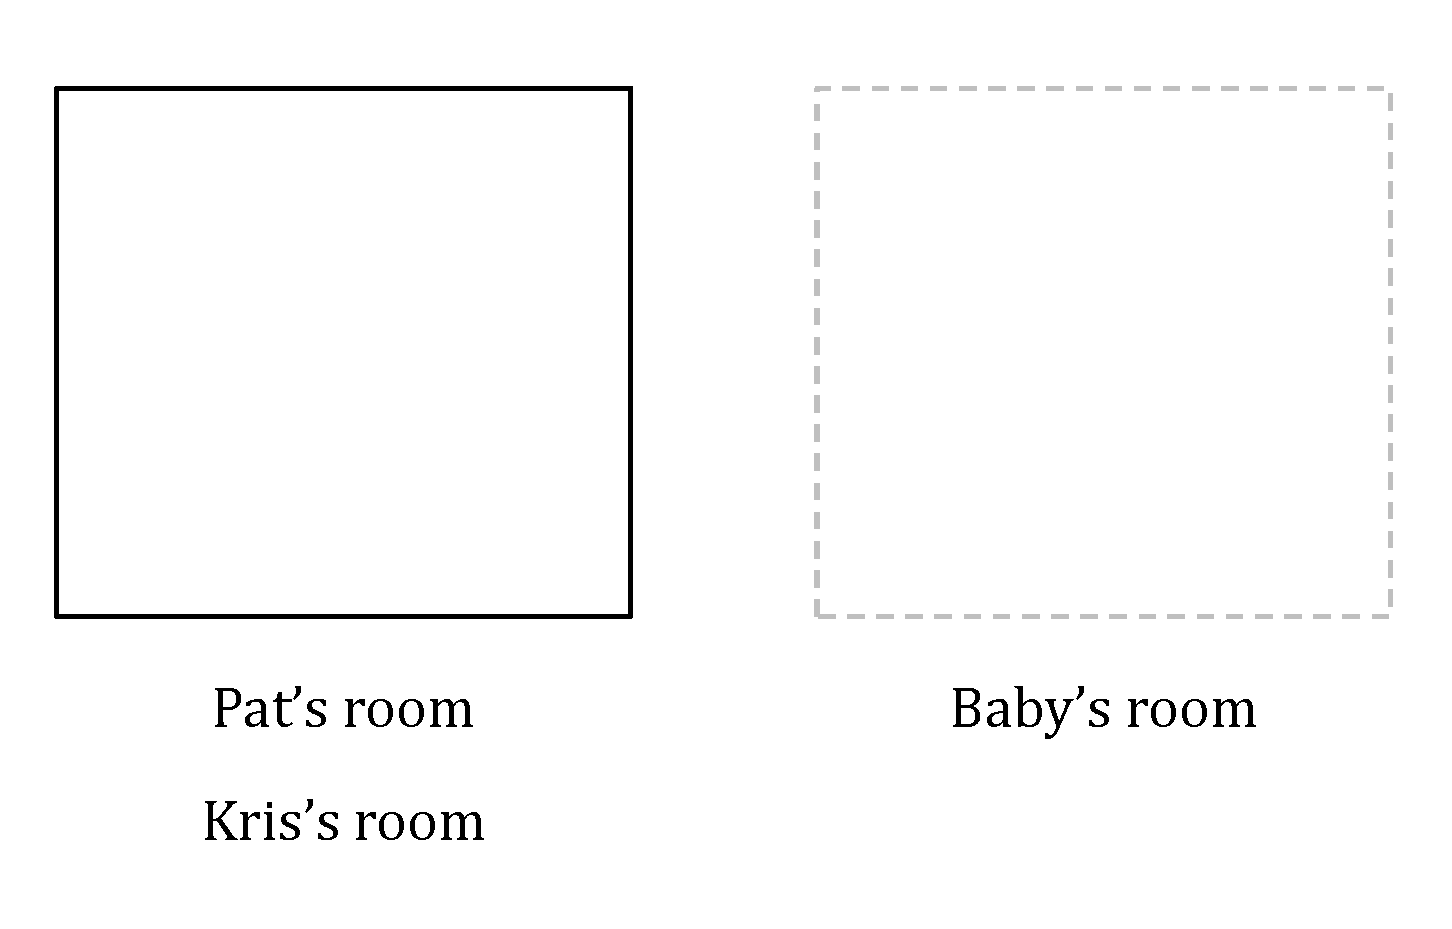
\includegraphics[width=0.6\textwidth]{res/room2_cropped.pdf}
		\end{figure}
	\end{frame}
	
	\begin{frame}
		\frametitle{Section \ref{sec:plot} : Plot}
		\framesubtitle{3. Sequence of events}
		\begin{itemize}
			\item They tried to evenly divide the room by tape in various ways.
		\end{itemize}
		\begin{figure}
			\centering
			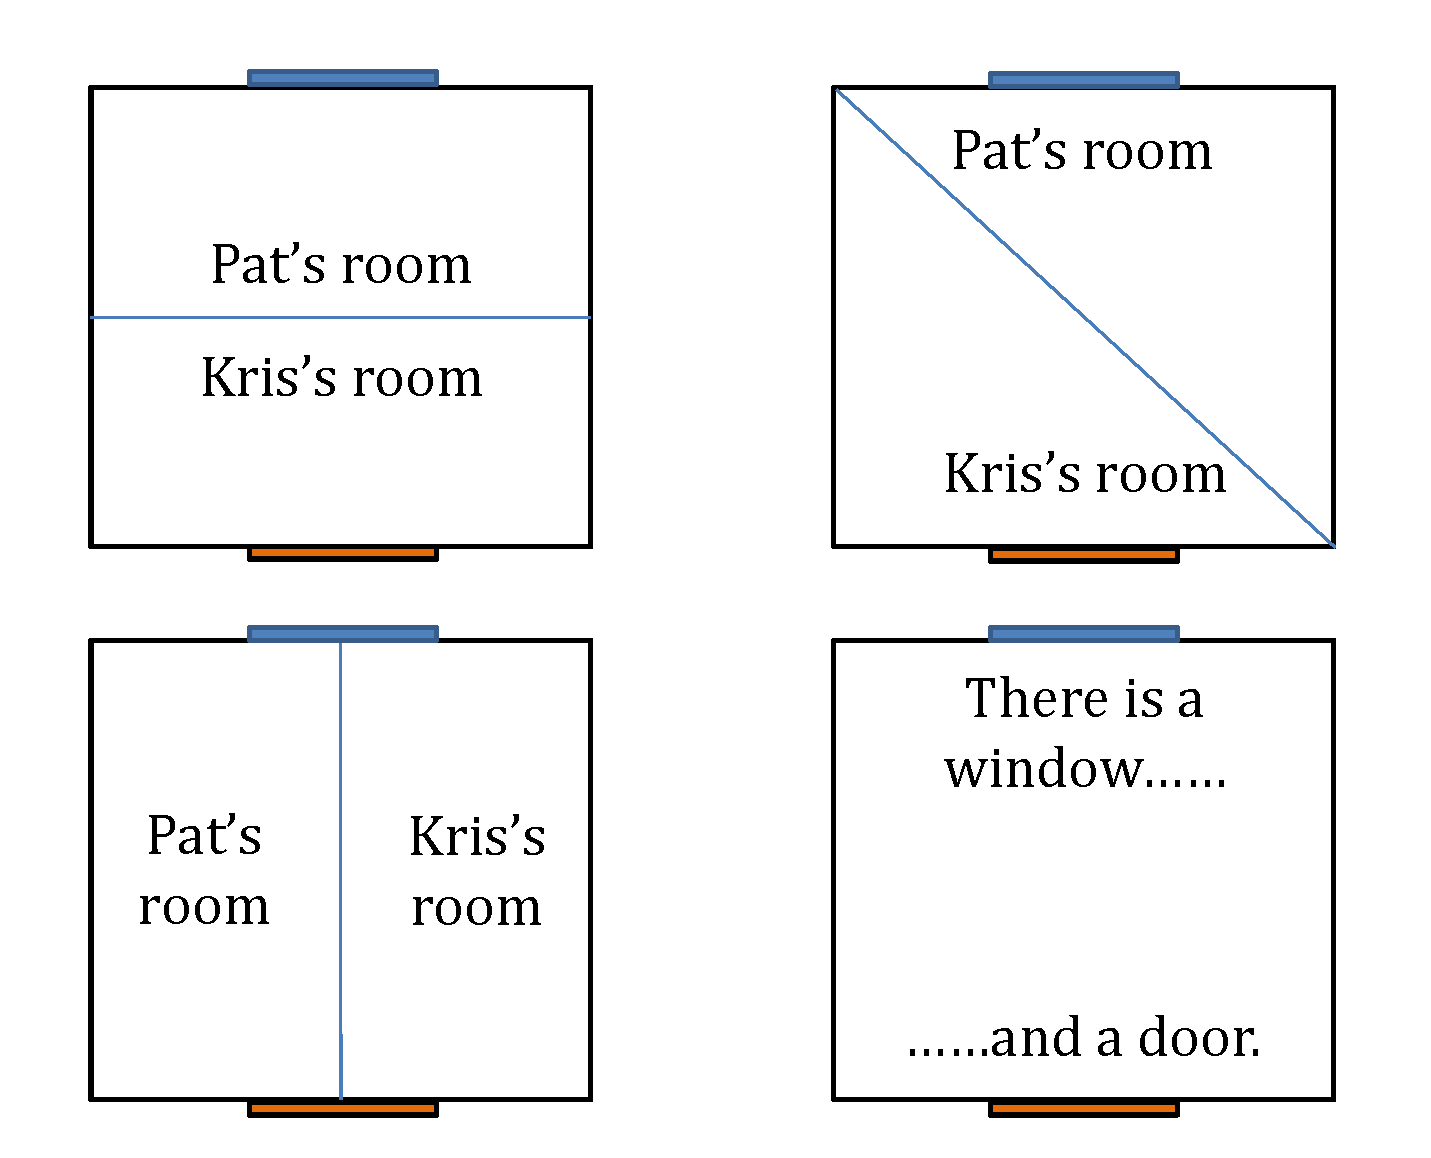
\includegraphics[width=0.7\textwidth]{res/room3_cropped.pdf}
		\end{figure}
	\end{frame}
	
	\begin{frame}
		\frametitle{Section \ref{sec:plot} : Plot}
		\framesubtitle{4. Climax}
		\begin{itemize}
			\item But moving all the things was a tiring job, so they sticked on the third version until the baby pulled all the tape.
			\item And then Mom announced something surprising......
		\end{itemize}
	\end{frame}
	
	\begin{frame}
		\frametitle{Section \ref{sec:plot} : Plot}
		\framesubtitle{5. Resolution}
		\begin{itemize}
			\item ......{\color{cyan} a bunk bed}.
			\item and Pat mentions {\bf ``......because our big square room is the very best shape!"}
		\end{itemize}
		\begin{figure}
			\centering
			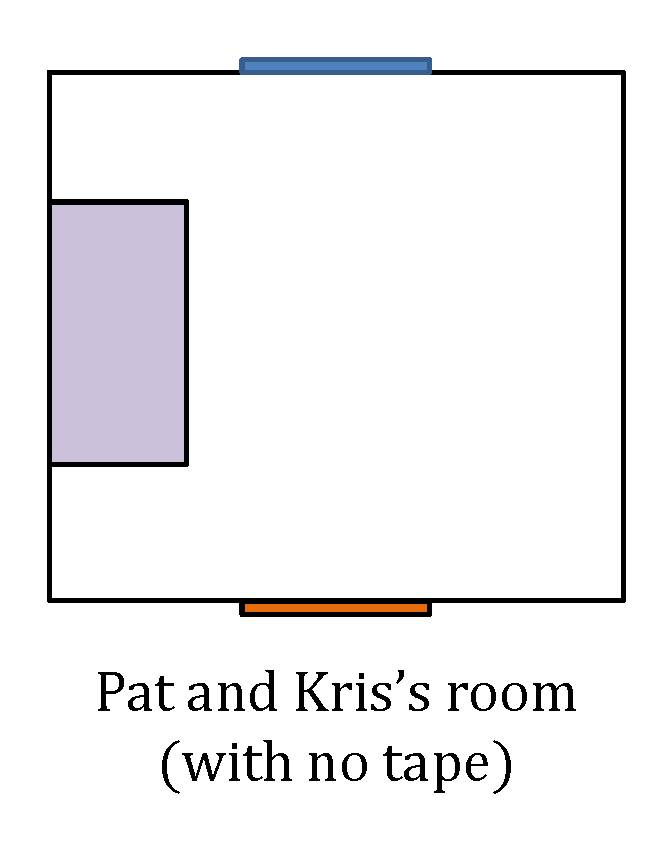
\includegraphics[width=0.4\textwidth]{res/room4_cropped.pdf}
		\end{figure}
	\end{frame}
	
	\begin{frame}
		\frametitle{Section \ref{sec:plot} : Plot}
		\framesubtitle{So what's the conflict?}
		\begin{itemize}
			\item In this story, Pat and Kris are trying to evenly divide the room, which is a fixed place.
			\item Thus, we can say that the conflict arises {\color{orange}between the siblings and the given circumstance}.
			\item Note that the circumstance was both posed and resolved by their Mom.
		\end{itemize}
	\end{frame}
	
	\section{Section 4 : Theme}\label{sec:theme}
	\begin{frame}
		\frametitle{Section \ref{sec:theme} : Theme}
		\begin{itemize}
			\item Most people will consent that there is no vivid moral in this cute little story.
			\item However, we can find that {\bf \color{violet} harmony between the siblings} was a crucial factor in the plot.
			\item It can be also inferred that parents usually try to resolve the problems of their children.
		\end{itemize}
	\end{frame}
	
	\section{Section 5 : Style}\label{sec:style}
	\begin{frame}
		\frametitle{Section \ref{sec:style} : Style}
		\begin{itemize}
			\item Pat refers herself as ``I'', indicating that the story has a {\bf first person point of view}.
			\item Pat also commonly uses the word ``we'', to refer herself and her sister, Kris.
		\end{itemize}
	\end{frame}
	
	%Which way makes the most sense?
	%Halves of squares
	\section{Section 6 : Scientific Concepts}\label{sec:science}
	\begin{frame}
		\frametitle{Section \ref{sec:science} : Scientific Concepts}
		\begin{itemize}
			\item {\bf Geometry!}
			\item The story mainly points out of the concept of {\bf evenly dividing}.
		\end{itemize}
	\end{frame}
	
	\begin{frame}
		\frametitle{Section \ref{sec:science} : Scientific Concepts}
		\begin{itemize}
			\item There are infinite ways to divide the square room in half.
			\item Some may be symmetric, others may not.
			\item It is symmetric only if......when?
		\end{itemize}
	\end{frame}
	
	\begin{frame}
		\frametitle{Section \ref{sec:science} : Scientific Concepts}
		\begin{itemize}
			\item Then, what is your best way to evenly divide the room? 
			\item Feel free to answer.
		\end{itemize}
	\end{frame}
	
	\begin{frame}
		\centering
		Thank you.
	\end{frame}
	
\end{document}
